% FXGCF Construction Comparison -- supervisor follow-up deck
% Style mirrors the final/proposal presentations (Beamer, Madrid theme).
% Build: latexmk -pdf main.tex
%
% Purpose: respond to the supervisor's concern that the thesis's FX-adjusted
% global cycle factor (FXGCF) is almost perfectly correlated with the GCF, by
% comparing three constructions (plus a 2x2-completing control) on correlation
% with the GCF and on in-/out-of-sample predictive power.
\documentclass[10pt]{beamer}

\usetheme{Madrid}

% Thesis colour scheme (see thesis_palette.R), so the deck matches the figures.
\definecolor{thesisindigo}{HTML}{3333AB}
\definecolor{thesisteal}{HTML}{008493}
\definecolor{thesissage}{HTML}{4D9F8B}
\usecolortheme[named=thesisindigo]{structure}
\setbeamercolor{alerted text}{fg=thesisteal}

\usepackage[utf8]{inputenc}
\usepackage[T1]{fontenc}
\usepackage{amsmath,amssymb}
\usepackage{graphicx}
\usepackage{booktabs}
\usepackage{natbib}
\bibliographystyle{apalike}

% Notation (matches the thesis / other decks)
\newcommand{\CF}{\mathrm{CF}}
\newcommand{\FXCF}{\mathrm{FXCF}}
\newcommand{\GCF}{\mathrm{GCF}}
\newcommand{\FXGCF}{\mathrm{FXGCF}}
\newcommand{\GCP}{\mathrm{GCP}}
\newcommand{\rx}{\mathit{rx}}
\newcommand{\rxbar}{\overline{rx}}
\newcommand{\cyc}{c}
\newcommand{\cycbar}{\bar{c}}
\newcommand{\E}{\mathbb{E}}
\DeclareMathOperator{\Corr}{Corr}

\AtBeginSection[]{%
  \begin{frame}{Outline}
    \tableofcontents[currentsection]
  \end{frame}}

\title[FXGCF construction comparison]{Comparing Constructions of the\\
  FX-adjusted Global Cycle Factor (FXGCF)}
\author[Jan Heissenberger]{Jan Heissenberger\\
  Supervised by Giorgia Simion, Ph.D.}
\date{June 2026}

\begin{document}

\begin{frame}
  \titlepage
\end{frame}

\begin{frame}{Outline}
  \tableofcontents
\end{frame}

% ==========================================================================
\section{The Problem}

\begin{frame}{The issue: FXGCF $\approx$ GCF}
  In the current thesis the FX-adjusted global cycle factor
  ($\FXGCF$) and the global cycle factor ($\GCF$) correlate
  \alert{$0.99$} in our sample.
  \begin{itemize}
    \item \citet{dahlquist2013}, our template, report
      $\Corr(\FXGCF,\GCF)\approx \mathbf{0.50}$. The FX factor is supposed to
      carry distinct, currency-driven information.
    \item At $0.99$ correlation the FX adjustment adds little economic content.
  \end{itemize}
  \vfill
  \begin{block}{What this deck does}
    Build the FXGCF \alert{three different ways}, and ask, for each:
    \begin{enumerate}
      \item how correlated is it with the $\GCF$ (and with the others)?
      \item how does its predictive power change (IS and OOS)
    \end{enumerate}
    Then recommend a construction.
  \end{block}
\end{frame}

\begin{frame}{$\GCF$ vs $\FXGCF$ (current)}
  The local-currency $\GCF$ is built \alert{bottom-up}, the current $\FXGCF$ is
  built \alert{top-down}.
  \vfill
  \textbf{$\GCF$ -- bottom-up (aggregate of local factors)}
  \begin{equation*}
    \CF_{i,t}=\widehat{\rxbar}_{i,t+12}\bigl(\cyc^{(1)}_{i,t},\cycbar_{i,t}\bigr),
    \qquad
    \GCF_{t}=\sum_{i} w_{i,t}\,\CF_{i,t}
  \end{equation*}
  \textbf{$\FXGCF$ -- top-down (one regression on global aggregates)}
  \begin{equation*}
    \FXGCF_{t}=\widehat{\rxbar}^{\,\mathrm{USD}}_{t+12}
      \Bigl(\underbrace{\textstyle\sum_i w_{i,t}\cyc^{(1)}_{i,t}}_{\bar c^{(1)}_t},\;
            \underbrace{\textstyle\sum_i w_{i,t}\cycbar_{i,t}}_{\bar{\cycbar}_t}\Bigr)
  \end{equation*}
  \vfill
  The top-down FXGCF is a fitted value on \emph{the very same} GDP-weighted
  cycle aggregates that drive $\GCF$. Therefore, it is collinear with $\GCF$ almost by
  construction.
\end{frame}

% ==========================================================================
\section{Three Constructions}

\begin{frame}{Three ways to build the FXGCF}
  All use the same cycle predictors and the US-dollar excess return
  $\rxbar^{\,\mathrm{USD}}$; they differ in \alert{construction} (top-down vs
  bottom-up) and \alert{weighting} (GDP vs $1/n$).
  \vspace{0.5ex}
  \begin{enumerate}
    \item[\textbf{M1}] \textbf{Top-down, GDP} \emph{(current)}: regress the
      GDP-weighted USD return on the GDP-weighted cycle aggregates.
    \item[\textbf{M2}] \textbf{Top-down, $1/n$}: same regression, but
      equal-weight countries into the aggregates.
    \item[\textbf{M3}] \textbf{Bottom-up, GDP}: build a \emph{local} FX cycle
      factor $\FXCF_{i}$ per country, then GDP-weight --
      \emph{exactly the $\GCF$ recipe, with the USD return on the left}.
  \[
    \FXCF_{i,t}=\widehat{\rxbar}^{\,\mathrm{USD}}_{i,t+12}
      \bigl(\cyc^{(1)}_{i,t},\cycbar_{i,t}\bigr),
    \qquad
    \FXGCF^{\mathrm{BU}}_{t}=\sum_i w_{i,t}\,\FXCF_{i,t}
  \]
    \item[\alert{M4}] \textbf{Bottom-up, $1/n$}: control method for completeness. To tell whether decoupling comes from weighting or TD/BU choice
  \end{enumerate}

  \vspace{-0.5ex}
\end{frame}

\begin{frame}{Definition}
      Let $w_{i,t}$ be GDP weights ($\sum_i w_{i,t}=1$) and $n_t$ the number of
  countries at $t$. Cycle predictors $\cyc^{(1)}_{i,t}$ (1y) and
  $\cycbar_{i,t}$ (average of the non-1y cycles).
  \begin{description}
    \item[M1 TD-GDP] $\FXGCF=\widehat{\rxbar}^{\,\mathrm{USD}}\!\left(\sum_i w_i\cyc^{(1)}_i,\ \sum_i w_i\cycbar_i\right)$, LHS $\sum_i w_i\rxbar^{\,\mathrm{USD}}_i$.
    \item[M2 TD-$1/n$] as M1 with $w_i\!\to\!1/n_t$ in all three aggregates.
    \item[M3 BU-GDP] $\FXCF_i=\widehat{\rxbar}^{\,\mathrm{USD}}_i(\cyc^{(1)}_i,\cycbar_i)$; $\FXGCF=\sum_i w_i\FXCF_i$.
    \item[M4 BU-$1/n$] $\FXGCF=\frac{1}{n_t}\sum_i\FXCF_i$.
  \end{description}
\end{frame}

\section{Results}
\begin{frame}{Results}
  \centering
  % fx_t1_summary -- master comparison of FXGCF constructions (build_comparison.R)
\setlength{\tabcolsep}{5pt}
\resizebox{\linewidth}{!}{%
\begin{tabular}{l l c c c c c}
  \toprule
  Construction & Weights & $\Corr(\cdot,\GCF)$ & $\overline{R^2}_{\text{IS}}$ & $|t|\!>\!1.96$ & pooled $R^2_{\text{oos}}$ & OOS$^{+}$ \\
  \midrule
  \multicolumn{7}{@{}l}{\textit{FX-adjusted global cycle factor (FXGCF)}}\\
  top-down (current) & GDP & $0.99$ & $0.101$ & 5/11 & $0.010$ & 9/11 \\
  top-down & 1/n & $0.95$ & $0.109$ & 6/11 & $0.033$ & 8/11 \\
  bottom-up & GDP & $0.81$ & $0.143$ & 10/11 & $0.021$ & 6/11 \\
  bottom-up & 1/n & $0.76$ & $0.140$ & 10/11 & $0.016$ & 6/11 \\
  \midrule
  \multicolumn{7}{@{}l}{\textit{Reference}}\\
  GCF (local-currency) & GDP & $1.00$ & $0.086$ & 4/11 & $-0.070$ & 2/11 \\
  \bottomrule
\end{tabular}}\\[0.8ex]
{\scriptsize\begin{minipage}{0.97\linewidth}
All factors predict the US-dollar excess return $\rxbar^{\,\mathrm{USD}}_{i,t+12}$. $\Corr(\cdot,\GCF)$ is the full-sample correlation with the GCF (n=412 months); $\overline{R^2}_{\text{IS}}$ is the cross-country mean in-sample $R^2$; pooled $R^2_{\text{oos}}$ is the Campbell--Thompson statistic against the recursive prevailing mean (doubly out-of-sample); OOS$^{+}$ counts markets with positive $R^2_{\text{oos}}$. Dahlquist--Hasseltoft (2013) report $\Corr(\text{FXGCP},\GCP)\approx0.50$.
\end{minipage}}

\end{frame}

\begin{frame}{Correlation matrix}
  \centering
  % fx_t2_corr -- correlation matrix of GCF and FXGCF constructions
\resizebox{\linewidth}{!}{%
\begin{tabular}{lccccc}
  \toprule
  & \rotatebox{45}{GCF} & \rotatebox{45}{TD - GDP (current)} & \rotatebox{45}{TD - 1/n} & \rotatebox{45}{BU - GDP} & \rotatebox{45}{BU - 1/n} \\
  \midrule
  GCF & $1.00$ &  &  &  &  \\
  TD - GDP (current) & $0.99$ & $1.00$ &  &  &  \\
  TD - 1/n & $0.95$ & $0.97$ & $1.00$ &  &  \\
  BU - GDP & $0.81$ & $0.85$ & $0.85$ & $1.00$ &  \\
  BU - 1/n & $0.76$ & $0.81$ & $0.87$ & $0.97$ & $1.00$ \\
  \bottomrule
\end{tabular}}
\\[1ex]
  {\scriptsize The bottom-up pair (M3, M4) correlate $0.96$ with each other but
   only $0.73$--$0.78$ with $\GCF$; the top-down pair (M1, M2) sit at
   $0.94$--$0.99$ with $\GCF$.}
\end{frame}

\begin{frame}{In-sample $R^2$ by country}
  \centering
  % fx_t3_is_r2 -- per-country in-sample R^2 (rx_USD ~ factor)
\setlength{\tabcolsep}{5pt}
\resizebox{\linewidth}{!}{%
\begin{tabular}{l c c c c c c}
  \toprule
  Country & local CF & GCF & TD-GDP & TD-1/n & BU-GDP & BU-1/n \\
  \midrule
  Belgium & $0.032$ & $0.048$ & $0.068$ & $0.085$ & $0.138$ & $0.144$ \\
  Germany & $0.065$ & $0.050$ & $0.071$ & $0.084$ & $0.147$ & $0.147$ \\
  France & $0.083$ & $0.050$ & $0.070$ & $0.087$ & $0.137$ & $0.145$ \\
  Italy & $0.109$ & $0.041$ & $0.054$ & $0.081$ & $0.077$ & $0.107$ \\
  Netherlands & $0.011$ & $0.050$ & $0.070$ & $0.084$ & $0.145$ & $0.146$ \\
  Switzerland & $0.146$ & $0.044$ & $0.066$ & $0.070$ & $0.169$ & $0.140$ \\
  UK & $0.114$ & $0.070$ & $0.077$ & $0.094$ & $0.049$ & $0.067$ \\
  Sweden & $0.098$ & $0.074$ & $0.092$ & $0.117$ & $0.091$ & $0.114$ \\
  Canada & $0.114$ & $0.126$ & $0.148$ & $0.167$ & $0.136$ & $0.149$ \\
  Japan & $0.000$ & $0.002$ & $0.009$ & $0.001$ & $0.064$ & $0.032$ \\
  US & $0.326$ & $0.326$ & $0.324$ & $0.298$ & $0.420$ & $0.363$ \\
  \bottomrule
\end{tabular}}\\[0.6ex]
{\scriptsize In-sample $R^2$ of $\rxbar^{\,\mathrm{USD}}_{i,t+12}\sim$ factor, per market.}

\end{frame}

\begin{frame}{Out-of-sample $R^2_{\mathrm{oos}}$ by country}
  \centering
  % fx_t4_oos_r2 -- per-country Campbell-Thompson R^2_oos (rx_USD ~ factor_oos)
\setlength{\tabcolsep}{5pt}
\resizebox{\linewidth}{!}{%
\begin{tabular}{l c c c c c}
  \toprule
  Country & GCF & TD-GDP & TD-1/n & BU-GDP & BU-1/n \\
  \midrule
  Belgium & $-0.082$ & $0.002$ & $0.009$ & $0.064$ & $0.066$ \\
  Germany & $-0.080$ & $0.002$ & $0.011$ & $0.067$ & $0.071$ \\
  France & $-0.081$ & $0.001$ & $0.012$ & $0.065$ & $0.067$ \\
  Italy & $-0.070$ & $-0.027$ & $-0.018$ & $0.065$ & $0.059$ \\
  Netherlands & $-0.079$ & $0.006$ & $0.017$ & $0.063$ & $0.067$ \\
  Switzerland & $-0.090$ & $0.114$ & $0.094$ & $-0.120$ & $-0.122$ \\
  UK & $-0.073$ & $0.007$ & $0.044$ & $-0.004$ & $-0.015$ \\
  Sweden & $-0.107$ & $0.029$ & $0.097$ & $-0.017$ & $-0.024$ \\
  Canada & $0.016$ & $0.109$ & $0.181$ & $-0.051$ & $-0.077$ \\
  Japan & $-0.049$ & $-0.191$ & $-0.158$ & $0.027$ & $0.024$ \\
  US & $0.066$ & $0.040$ & $-0.099$ & $-0.148$ & $-0.175$ \\
  \bottomrule
\end{tabular}}\\[0.6ex]
{\scriptsize Campbell--Thompson $R^2_{\text{oos}}$ vs. the recursive prevailing mean, per market.}

\end{frame}

\begin{frame}{Conclusion}
  \begin{enumerate}
    \item The $0.99$ correlation is an \alert{artefact of the top-down
      construction}, not evidence that FX information is absent: the current
      FXGCF is a fitted value on the same global cycle aggregates as $\GCF$.
    \item Rebuilding it \alert{bottom-up} (M3) cuts $\Corr(\cdot,\GCF)$ to $0.78$, lifts in-sample $R^2$ to
      $14.3\%$ (10/11 markets), and stays positive out of sample.
  \end{enumerate}
  \vfill
  \raggedright \textbf{Proposed change to the thesis:} replace the top-down FXGCF
  with the bottom-up GDP-weighted FXGCF (\textbf{M3}). Put top-down approach (\textbf{M2}) in the robustness section.
\end{frame}

\begin{frame}{References}
  \small
  \bibliography{references}
\end{frame}
\end{document}

% ==========================================================================
\section{Results: Correlation}

\begin{frame}{Correlation with the GCF: construction is the lever}
  \begin{columns}[T]
    \begin{column}{0.56\textwidth}
      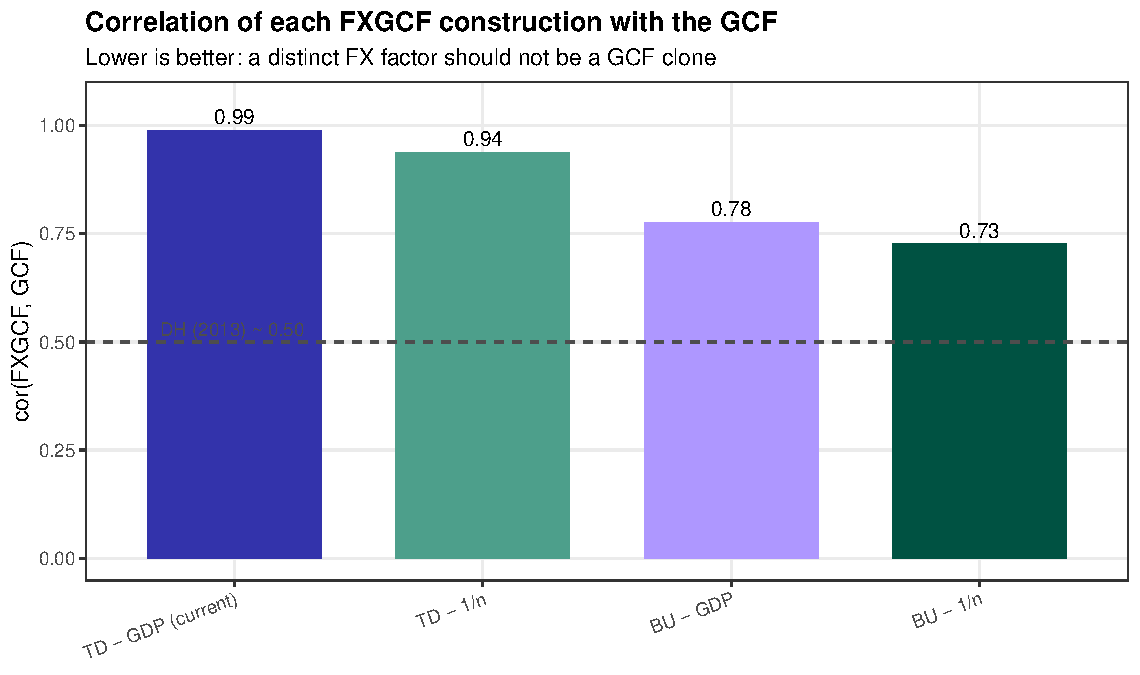
\includegraphics[width=\linewidth]{figures/fx_f2_corr_gcf.pdf}
    \end{column}
    \begin{column}{0.44\textwidth}
      \begin{itemize}
        \item Current (TD-GDP): $\rho=\mathbf{0.99}$.
        \item Equal-weighting alone barely helps: TD-$1/n$ still
          $\rho=0.94$.
        \item Going \alert{bottom-up} nearly halves the gap to $\GCF$:
          BU-GDP $\rho=\mathbf{0.78}$, BU-$1/n$ $\rho=0.73$.
      \end{itemize}
      \vfill
      \textbf{Read of the $2\times2$:} the \emph{top-down vs bottom-up} choice
      moves $\rho$ far more than the weighting scheme. None reach DH's $0.50$
      (same predictors throughout) -- see caveats.
    \end{column}
  \end{columns}
\end{frame}

\begin{frame}{The same picture over time}
  \centering
  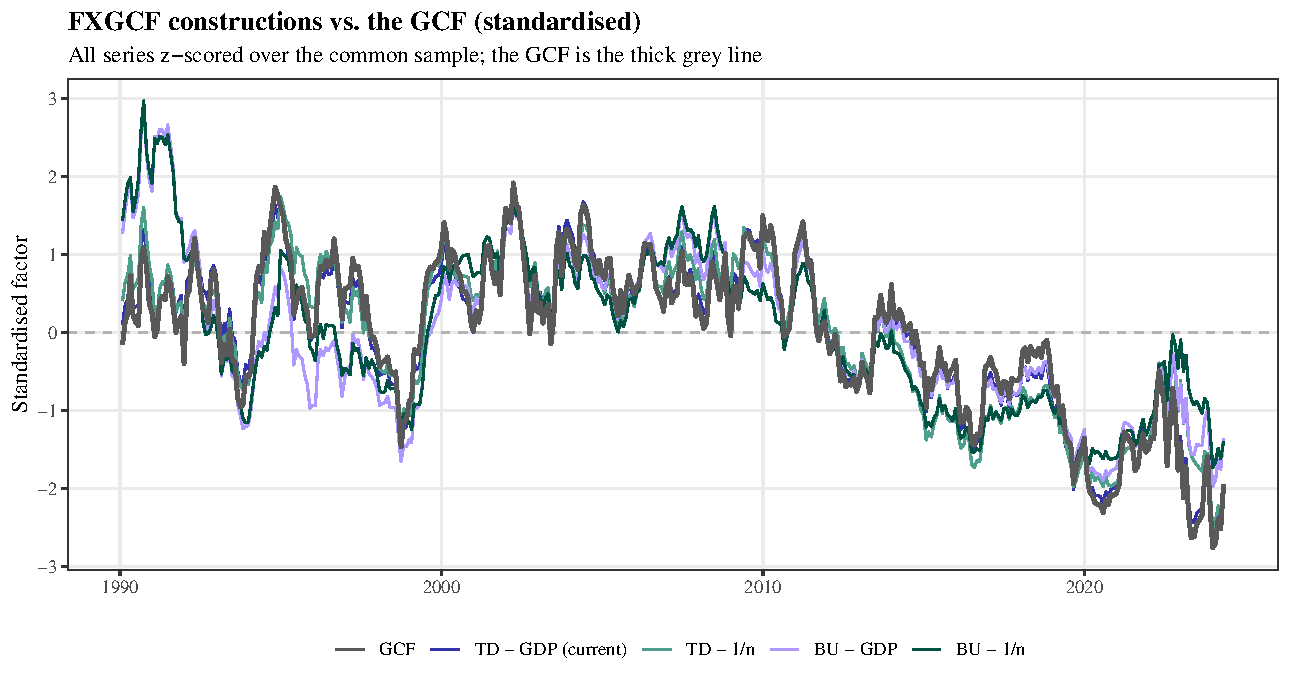
\includegraphics[width=0.92\linewidth]{figures/fx_f1_timeseries.pdf}\\[0.5ex]
  {\scriptsize The current FXGCF (indigo) is hidden under the $\GCF$ (thick
   grey): they are visually the same series. The bottom-up factors
   (lavender/forest) depart from the $\GCF$ in the late-1990s, the euro crisis,
   and post-2020.}
\end{frame}

% ==========================================================================
\section{Results: Predictive Power}

\begin{frame}{In-sample: the less-collinear factor predicts \emph{better}}
  \begin{columns}[T]
    \begin{column}{0.56\textwidth}
      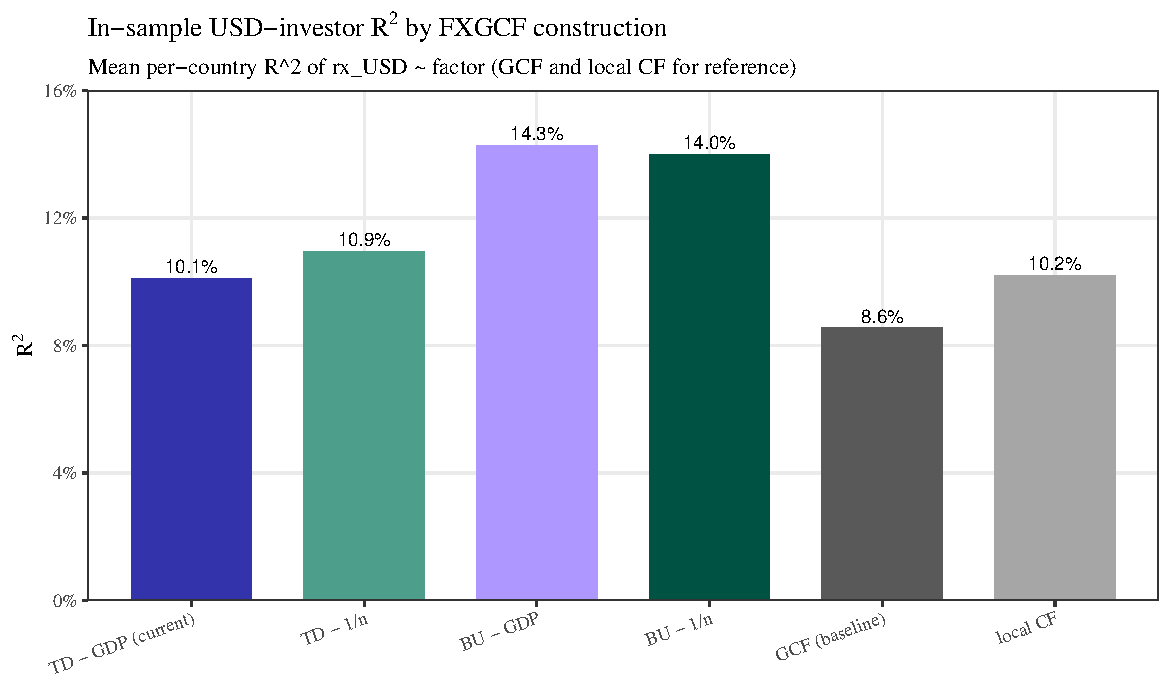
\includegraphics[width=\linewidth]{figures/fx_f4_is_r2.pdf}
    \end{column}
    \begin{column}{0.44\textwidth}
      USD-investor return $\rxbar^{\,\mathrm{USD}}_{i,t+12}\sim$ factor, per
      market (Newey--West HAC).
      \begin{itemize}
        \item Mean $R^2$: current \textbf{9.5\%} $\to$ bottom-up
          \textbf{14.3\%}.
        \item Significant ($|t|>1.96$) in \textbf{10/11} markets for BU-GDP vs
          only \textbf{4/11} for the current factor.
        \item Beats both the $\GCF$ ($8.0\%$) and the local $\CF$ ($10.0\%$)
          baselines.
      \end{itemize}
      \alert{No trade-off:} the construction that decouples from $\GCF$ is also
      the more powerful one.
    \end{column}
  \end{columns}
\end{frame}

\begin{frame}{Out-of-sample: all beat the unadjusted $\GCF$}
  \begin{columns}[T]
    \begin{column}{0.56\textwidth}
      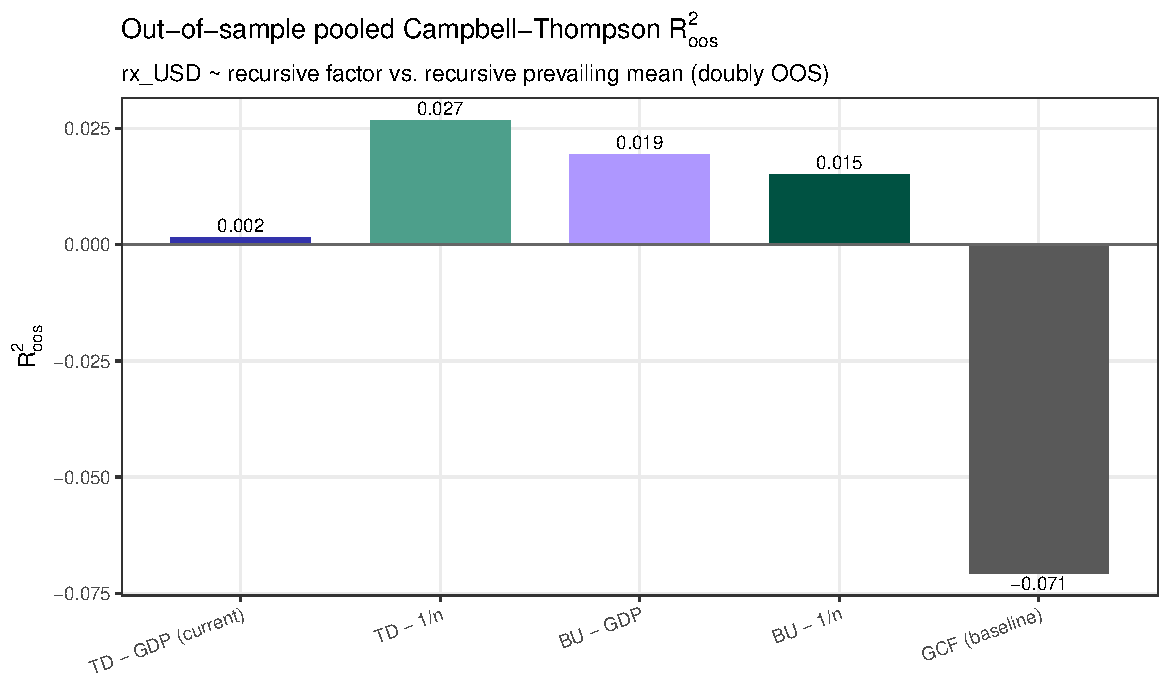
\includegraphics[width=\linewidth]{figures/fx_f5_oos_r2.pdf}
    \end{column}
    \begin{column}{0.44\textwidth}
      Pooled Campbell--Thompson $R^2_{\mathrm{oos}}$, fully recursive (the factor
      \emph{and} the forecast respect time $t$).
      \begin{itemize}
        \item Unadjusted $\GCF$ on USD returns: \alert{$-0.071$} -- worse than
          the prevailing mean.
        \item \textbf{Every} FX construction turns it positive.
        \item Current TD-GDP is the \emph{weakest} ($+0.002$); TD-$1/n$
          ($+0.027$) and BU-GDP ($+0.019$) lead.
      \end{itemize}
      OOS is noisier than IS: BU wins across the euro area, the top-down/equal
      factors win in CA/SE/CH (see appendix).
    \end{column}
  \end{columns}
\end{frame}

\begin{frame}{Everything in one table}
  \centering
  % fx_t1_summary -- master comparison of FXGCF constructions (build_comparison.R)
\setlength{\tabcolsep}{5pt}
\resizebox{\linewidth}{!}{%
\begin{tabular}{l l c c c c c}
  \toprule
  Construction & Weights & $\Corr(\cdot,\GCF)$ & $\overline{R^2}_{\text{IS}}$ & $|t|\!>\!1.96$ & pooled $R^2_{\text{oos}}$ & OOS$^{+}$ \\
  \midrule
  \multicolumn{7}{@{}l}{\textit{FX-adjusted global cycle factor (FXGCF)}}\\
  top-down (current) & GDP & $0.99$ & $0.101$ & 5/11 & $0.010$ & 9/11 \\
  top-down & 1/n & $0.95$ & $0.109$ & 6/11 & $0.033$ & 8/11 \\
  bottom-up & GDP & $0.81$ & $0.143$ & 10/11 & $0.021$ & 6/11 \\
  bottom-up & 1/n & $0.76$ & $0.140$ & 10/11 & $0.016$ & 6/11 \\
  \midrule
  \multicolumn{7}{@{}l}{\textit{Reference}}\\
  GCF (local-currency) & GDP & $1.00$ & $0.086$ & 4/11 & $-0.070$ & 2/11 \\
  \bottomrule
\end{tabular}}\\[0.8ex]
{\scriptsize\begin{minipage}{0.97\linewidth}
All factors predict the US-dollar excess return $\rxbar^{\,\mathrm{USD}}_{i,t+12}$. $\Corr(\cdot,\GCF)$ is the full-sample correlation with the GCF (n=412 months); $\overline{R^2}_{\text{IS}}$ is the cross-country mean in-sample $R^2$; pooled $R^2_{\text{oos}}$ is the Campbell--Thompson statistic against the recursive prevailing mean (doubly out-of-sample); OOS$^{+}$ counts markets with positive $R^2_{\text{oos}}$. Dahlquist--Hasseltoft (2013) report $\Corr(\text{FXGCP},\GCP)\approx0.50$.
\end{minipage}}

  \vfill
  {\scriptsize Bottom-up cuts $\Corr(\cdot,\GCF)$ from $0.99$ to $0.78$ \emph{and}
   raises in-sample power and breadth (10/11 markets significant); all four FX
   variants beat the $-0.071$ OOS of the unadjusted $\GCF$.}
\end{frame}

% ==========================================================================
\section{Recommendation}

\begin{frame}{Recommendation: adopt the bottom-up GDP factor (M3)}
  \begin{block}{Why M3 (bottom-up, GDP-weighted)}
    \begin{enumerate}
      \item \textbf{Symmetric \& defensible:} identical recipe to the $\GCF$,
        just the US-dollar return on the left -- one sentence to describe.
      \item \textbf{Decouples from $\GCF$:} $\rho$ falls $0.99\to0.78$, so the
        factor carries genuinely different information.
      \item \textbf{Strongest in sample:} mean $R^2=14.3\%$, significant in
        10/11 markets.
      \item \textbf{Survives out of sample:} pooled $R^2_{\mathrm{oos}}=+0.019$,
        well above the $\GCF$'s $-0.071$.
    \end{enumerate}
  \end{block}
  \footnotesize
  \textbf{If the priority is purely OOS accuracy}, TD-$1/n$ edges it
  ($+0.027$) but stays $0.94$-correlated with $\GCF$ -- it does not fix the
  original concern. M3 is the better all-round answer.
\end{frame}

\begin{frame}{Honest caveats \& outlook}
  \begin{itemize}
    \item \textbf{None reaches DH's $0.50$.} All four constructions reuse the
      \emph{same bond-cycle predictors} $(\cyc^{(1)},\cycbar)$; they can only
      re-weight that common signal, so a floor on $\rho$ with $\GCF$ remains.
    \item \textbf{To truly decouple} the FX factor one likely needs a
      \alert{currency-specific predictor} in the menu -- e.g.\ the short-rate
      differential / carry $\bigl(y^{(1)}_{i}-y^{(1)}_{\mathrm{US}}\bigr)$,
      which drives the predictable part of the currency return. This is the
      natural next step and matches \emph{why} DH's factor is distinct.
    \item \textbf{OOS ranking is sample-dependent} (euro area vs CA/SE/CH); the
      in-sample and correlation results are the robust ones.
  \end{itemize}
  \vfill
  \begin{block}{Bottom line}
    Switching the FXGCF from top-down to bottom-up makes it a genuinely distinct,
    and more powerful, factor -- without adding a single new input.
  \end{block}
\end{frame}

\begin{frame}{Conclusion}
  \begin{enumerate}
    \item The $0.99$ correlation is an \alert{artefact of the top-down
      construction}, not evidence that FX information is absent: the current
      FXGCF is a fitted value on the same global cycle aggregates as $\GCF$.
    \item Rebuilding it \alert{bottom-up} (M3) -- the $\GCF$ recipe on USD
      returns -- cuts $\Corr(\cdot,\GCF)$ to $0.78$, lifts in-sample $R^2$ to
      $14.3\%$ (10/11 markets), and stays positive out of sample.
    \item Reaching DH's $\approx 0.50$ would require adding a currency-specific
      predictor; that is the recommended extension.
  \end{enumerate}
  \vfill
  \centering\textit{Proposed change to the thesis: replace the top-down FXGCF
  with the bottom-up GDP-weighted FXGCF.}
\end{frame}



% ==========================================================================
\appendix
\section{Appendix}

\begin{frame}{Appendix: correlation matrix}
  \centering
  % fx_t2_corr -- correlation matrix of GCF and FXGCF constructions
\resizebox{\linewidth}{!}{%
\begin{tabular}{lccccc}
  \toprule
  & \rotatebox{45}{GCF} & \rotatebox{45}{TD - GDP (current)} & \rotatebox{45}{TD - 1/n} & \rotatebox{45}{BU - GDP} & \rotatebox{45}{BU - 1/n} \\
  \midrule
  GCF & $1.00$ &  &  &  &  \\
  TD - GDP (current) & $0.99$ & $1.00$ &  &  &  \\
  TD - 1/n & $0.95$ & $0.97$ & $1.00$ &  &  \\
  BU - GDP & $0.81$ & $0.85$ & $0.85$ & $1.00$ &  \\
  BU - 1/n & $0.76$ & $0.81$ & $0.87$ & $0.97$ & $1.00$ \\
  \bottomrule
\end{tabular}}
\\[1ex]
  {\scriptsize The bottom-up pair (M3, M4) correlate $0.96$ with each other but
   only $0.73$--$0.78$ with $\GCF$; the top-down pair (M1, M2) sit at
   $0.94$--$0.99$ with $\GCF$.}
\end{frame}

\begin{frame}{Appendix: correlation heatmap}
  \centering
  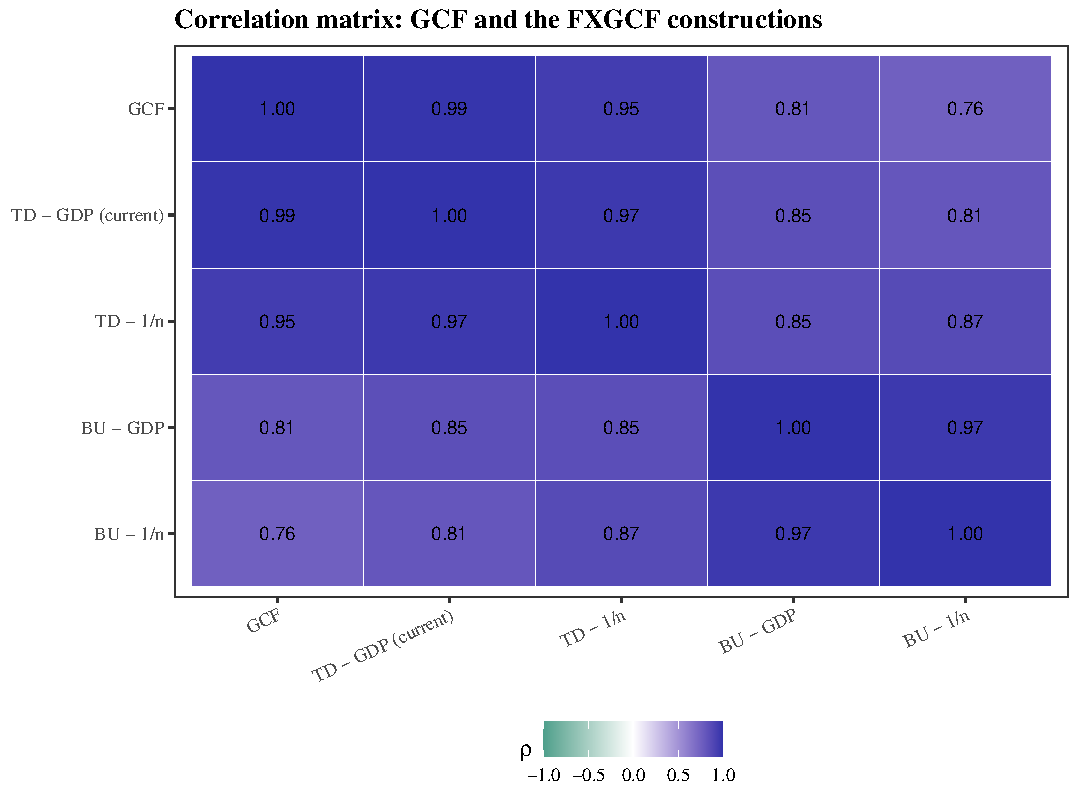
\includegraphics[width=0.74\linewidth]{figures/fx_f3_corr_heatmap.pdf}
\end{frame}

\begin{frame}{Appendix: in-sample $R^2$ by country}
  \centering
  % fx_t3_is_r2 -- per-country in-sample R^2 (rx_USD ~ factor)
\setlength{\tabcolsep}{5pt}
\resizebox{\linewidth}{!}{%
\begin{tabular}{l c c c c c c}
  \toprule
  Country & local CF & GCF & TD-GDP & TD-1/n & BU-GDP & BU-1/n \\
  \midrule
  Belgium & $0.032$ & $0.048$ & $0.068$ & $0.085$ & $0.138$ & $0.144$ \\
  Germany & $0.065$ & $0.050$ & $0.071$ & $0.084$ & $0.147$ & $0.147$ \\
  France & $0.083$ & $0.050$ & $0.070$ & $0.087$ & $0.137$ & $0.145$ \\
  Italy & $0.109$ & $0.041$ & $0.054$ & $0.081$ & $0.077$ & $0.107$ \\
  Netherlands & $0.011$ & $0.050$ & $0.070$ & $0.084$ & $0.145$ & $0.146$ \\
  Switzerland & $0.146$ & $0.044$ & $0.066$ & $0.070$ & $0.169$ & $0.140$ \\
  UK & $0.114$ & $0.070$ & $0.077$ & $0.094$ & $0.049$ & $0.067$ \\
  Sweden & $0.098$ & $0.074$ & $0.092$ & $0.117$ & $0.091$ & $0.114$ \\
  Canada & $0.114$ & $0.126$ & $0.148$ & $0.167$ & $0.136$ & $0.149$ \\
  Japan & $0.000$ & $0.002$ & $0.009$ & $0.001$ & $0.064$ & $0.032$ \\
  US & $0.326$ & $0.326$ & $0.324$ & $0.298$ & $0.420$ & $0.363$ \\
  \bottomrule
\end{tabular}}\\[0.6ex]
{\scriptsize In-sample $R^2$ of $\rxbar^{\,\mathrm{USD}}_{i,t+12}\sim$ factor, per market.}

\end{frame}

\begin{frame}{Appendix: out-of-sample $R^2_{\mathrm{oos}}$ by country}
  \centering
  % fx_t4_oos_r2 -- per-country Campbell-Thompson R^2_oos (rx_USD ~ factor_oos)
\setlength{\tabcolsep}{5pt}
\resizebox{\linewidth}{!}{%
\begin{tabular}{l c c c c c}
  \toprule
  Country & GCF & TD-GDP & TD-1/n & BU-GDP & BU-1/n \\
  \midrule
  Belgium & $-0.082$ & $0.002$ & $0.009$ & $0.064$ & $0.066$ \\
  Germany & $-0.080$ & $0.002$ & $0.011$ & $0.067$ & $0.071$ \\
  France & $-0.081$ & $0.001$ & $0.012$ & $0.065$ & $0.067$ \\
  Italy & $-0.070$ & $-0.027$ & $-0.018$ & $0.065$ & $0.059$ \\
  Netherlands & $-0.079$ & $0.006$ & $0.017$ & $0.063$ & $0.067$ \\
  Switzerland & $-0.090$ & $0.114$ & $0.094$ & $-0.120$ & $-0.122$ \\
  UK & $-0.073$ & $0.007$ & $0.044$ & $-0.004$ & $-0.015$ \\
  Sweden & $-0.107$ & $0.029$ & $0.097$ & $-0.017$ & $-0.024$ \\
  Canada & $0.016$ & $0.109$ & $0.181$ & $-0.051$ & $-0.077$ \\
  Japan & $-0.049$ & $-0.191$ & $-0.158$ & $0.027$ & $0.024$ \\
  US & $0.066$ & $0.040$ & $-0.099$ & $-0.148$ & $-0.175$ \\
  \bottomrule
\end{tabular}}\\[0.6ex]
{\scriptsize Campbell--Thompson $R^2_{\text{oos}}$ vs. the recursive prevailing mean, per market.}

\end{frame}

\begin{frame}{Appendix: factor definitions}
  \footnotesize
  Let $w_{i,t}$ be GDP weights ($\sum_i w_{i,t}=1$) and $n_t$ the number of
  countries at $t$. Cycle predictors $\cyc^{(1)}_{i,t}$ (1y) and
  $\cycbar_{i,t}$ (average of the non-1y cycles).
  \begin{description}
    \item[M1 TD-GDP] $\FXGCF=\widehat{\rxbar}^{\,\mathrm{USD}}\!\left(\sum_i w_i\cyc^{(1)}_i,\ \sum_i w_i\cycbar_i\right)$, LHS $\sum_i w_i\rxbar^{\,\mathrm{USD}}_i$.
    \item[M2 TD-$1/n$] as M1 with $w_i\!\to\!1/n_t$ in all three aggregates.
    \item[M3 BU-GDP] $\FXCF_i=\widehat{\rxbar}^{\,\mathrm{USD}}_i(\cyc^{(1)}_i,\cycbar_i)$; $\FXGCF=\sum_i w_i\FXCF_i$.
    \item[M4 BU-$1/n$] $\FXGCF=\frac{1}{n_t}\sum_i\FXCF_i$.
  \end{description}
  \vfill
  All evaluated on G10 monthly data, 1990s--2026. In-sample: Newey--West HAC,
  per country (common 412-month sample). Out-of-sample: fully-recursive factors
  and forecasts, pooled Campbell--Thompson $R^2_{\mathrm{oos}}$ vs.\ the
  recursive prevailing mean (5y training minimum), scored on a \emph{common}
  $(\text{country},\text{month})$ sample so burn-ins cannot confound the ranking.
  Reproduce with \texttt{Rscript fxgcf\_comparison/build\_comparison.R}.
\end{frame}

\end{document}
